% -*- coding: utf-8; -*-

\chapter{Introduction}

So, to start with, could you provide me with more details about your research idea? What specific area in the field of programming languages are you interested in? What problem or question would you like your research to address?

Sure. I'll provide you with more details about our research idea. I will present you some background information so we can formulate an enthralling laconic research proposal for our target audience.

I am interested in Typing Mutable References. The main reference for the problem my research adresses is the Software Foundations series by Benjamin C. Pierce. The first two volumes, "Logical Foundations" and "Programming Language Foundations" gives a solid understanding of "functional programming, basic concepts of logic, computer-assisted theorem proving, and Coq." and also "the theory of programming languages, including operational semantics and static type systems." respectively. More specifically, the chapter "References" contains a very interesting implementation of mutable references in a Simply Typed Lambda Calculus (STLC) language that we take as an inspiration for condcting our study aroud typing mutable references.


The main idea behind our study is to
    - propose a different approach for the syntax definition of terms inside a Simply Typed Lambda Calculus (STLC) language.
    - redefine the operational semantics comprising our new term definition
    - Check if the standard type safety properties still hold (progress and preservation theorems).
    - Analyse both solutions (canonical and research) comparing simplicity, reasoning, understanding and proof implementations.


Naturally, when introducing mutable references in a language definition, we would consider the following terms (as described in the book Programming Language Foundations, chapter References):

```coq
(** *** Terms *)

(** Besides variables, abstractions, applications,
    natural-number-related terms, and [unit], we need four more sorts
    of terms in order to handle mutable references:

        t ::= ...              Terms
            | ref t              allocation
            | !t                 dereference
            | t := t             assignment
            | l                  location
*)

Inductive tm  : Type :=
    (* STLC with numbers: *)
    | tm_var    : string -> tm
    | tm_app    : tm -> tm -> tm
    | tm_abs    : string -> ty -> tm -> tm
    | tm_const  : nat -> tm
    | tm_succ    : tm -> tm
    | tm_pred    : tm -> tm
    | tm_mult    : tm -> tm -> tm
    | tm_if0  : tm -> tm -> tm -> tm
    (* New terms: *)
    | tm_unit   : tm
    | tm_ref    : tm -> tm
    | tm_deref  : tm -> tm
    | tm_assign : tm -> tm -> tm
    | tm_loc    : nat -> tm.
```


% \begin{figure}
% \centering
% 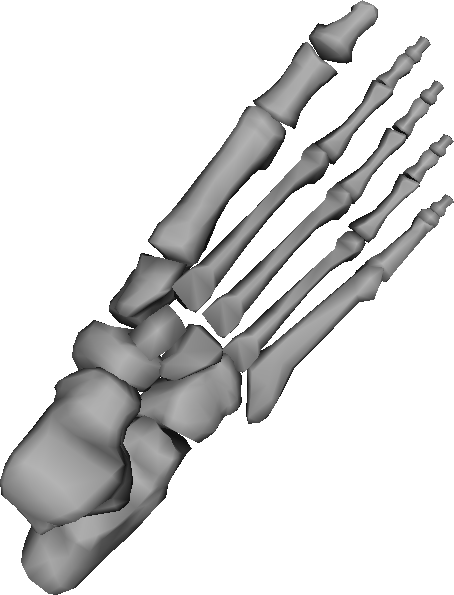
\includegraphics[width=0.45\textwidth]{pictures/image01.png}
% 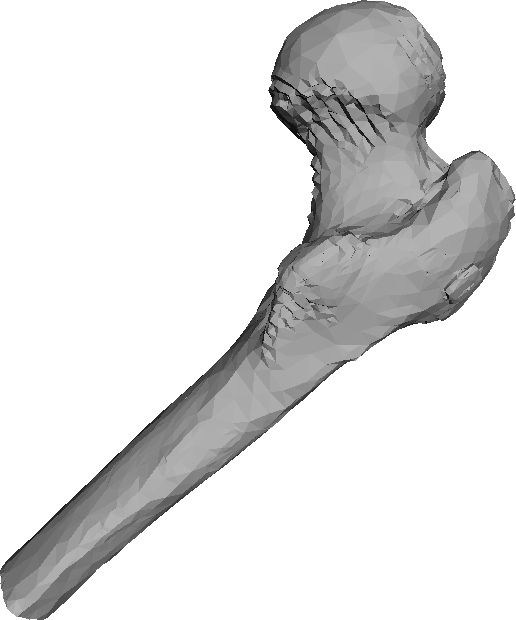
\includegraphics[width=0.45\textwidth]{pictures/image02.png}
% \caption{Meshes generated from medical data. Data obtained from the AIM$@$SHAPE Shape Repository \cite{AIMSHAPE}}
% \label{fig:example}
% \end{figure}


This document is structured as follows. In Chapter~\ref{cha:Previous Work} we present some previous work relevant to our problem. In Chapter~\ref{cha:Proposal} we explain our proposal. In Chapter~\ref{cha:Results} we show our results. Finally, in Chapter~\ref{cha:Conclusion} we present our conclusion and future work.


